\chapter{Durchführung}

Ausgehend von dem nun verfügbaren Datensatz, ist es möglich mit der Anwendung auf unser Problem zu beginnen.



\section{Aminosäurerest-Pseudopotential Spektrum}


\subsection{Quartile}
In einer ersten Analyse, wurde die Allgemeine Verteilung der \ac{APs} in Quartile erfasst. Dies wurde mit dem Skript \texttt{check\_energy\_quants.py} durchgeführt und die Ergebnisse in \ac{Abb} \ref{fig:quartiles_glob} und \ref{fig:quartiles_memb} dargestellt. 
%
\begin{figure}
\centering
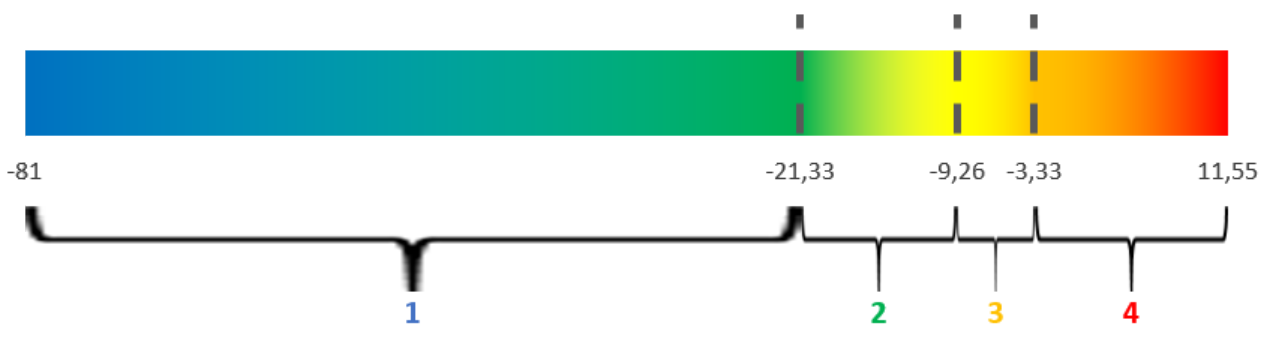
\includegraphics[width=.95\textwidth]{images/Quartil_glob.png}
\caption{Verteilung des Energiespektrums aller Energieprofile der globulären Proteine, in vier Perzentile, mit Grenzen.}
\label{fig:quartiles_glob}
\end{figure}

%new Quantile for globular:
%-81.2912287163
%-21.5377154868
%-9.50643383752
%-3.44146165978
%11.768577356
\begin{figure}
\centering
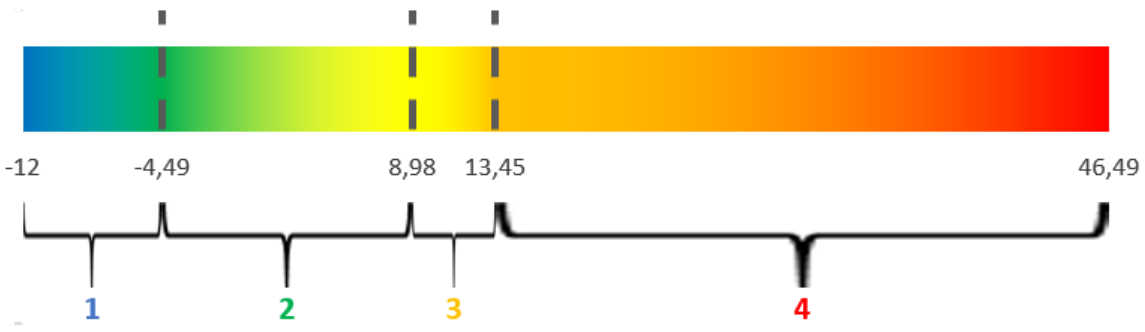
\includegraphics[width=.95\textwidth]{images/Quartil_memb.png}
\caption{Verteilung des Energiespektrums aller Energieprofile der Membran assoziierten Proteine, in vier Perzentile, mit Grenzen.}
\label{fig:quartiles_memb}
\end{figure}

%Quantile for membrane:
%-12.2373208162
%4.49279516205
%8.98564351117
%13.4598691639
%46.4967251975

In \ref{fig:quartiles_glob} werden die Quartile für alle globulären Proteine dargestellt, hierbei ist auffällig, dass das größte Quartil von -81 bis -22,21 geht und sich das kleinste Quartil von -9,26 bis -3,33 befindet. In \ref{fig:quartiles_memb} werden die Quartile aller alpha helicalen Proteine dargestellt, hier ist die relative Quartilgröße ähnlich. Doch es fällt auf, dass die obere und untere Grenze sich deutlich von \ref{fig:quartiles_glob} unterscheiden, denn die untere Grenze beginnt bei -12 anstelle von -81. Die obere Grenze hingegen reicht bis +46,49 anstelle von +11,5.

Aufgrund der Übersichtlichkeit und durch die geringe Anzahl an alpha helicalen \ac{EP}s, befasst sich diese Arbeit sich hauptsächlich mit globulären Proteinen.


\subsection{Spektrum aller Aminosäuren}
In einem weiteren Schritt wurde überprüft, ob und wie sich die \ac{AP} Verteilung zwischen den einzelnen Aminosäuren unterscheidet. Dafür wurde der gesamte Datensatz aus 132.098 globulären \ac{EP}s mit dem Skript \texttt{check\_aa\_energy\_range.py} analysiert. Das Skript lieferte die \ac{Abb} \ref{fig:energy_ranges}, welche zeigt, dass nicht alle Aminosäuren im gleichen Energie Spektrum zu finden sind. 


\begin{figure}
    \centering
    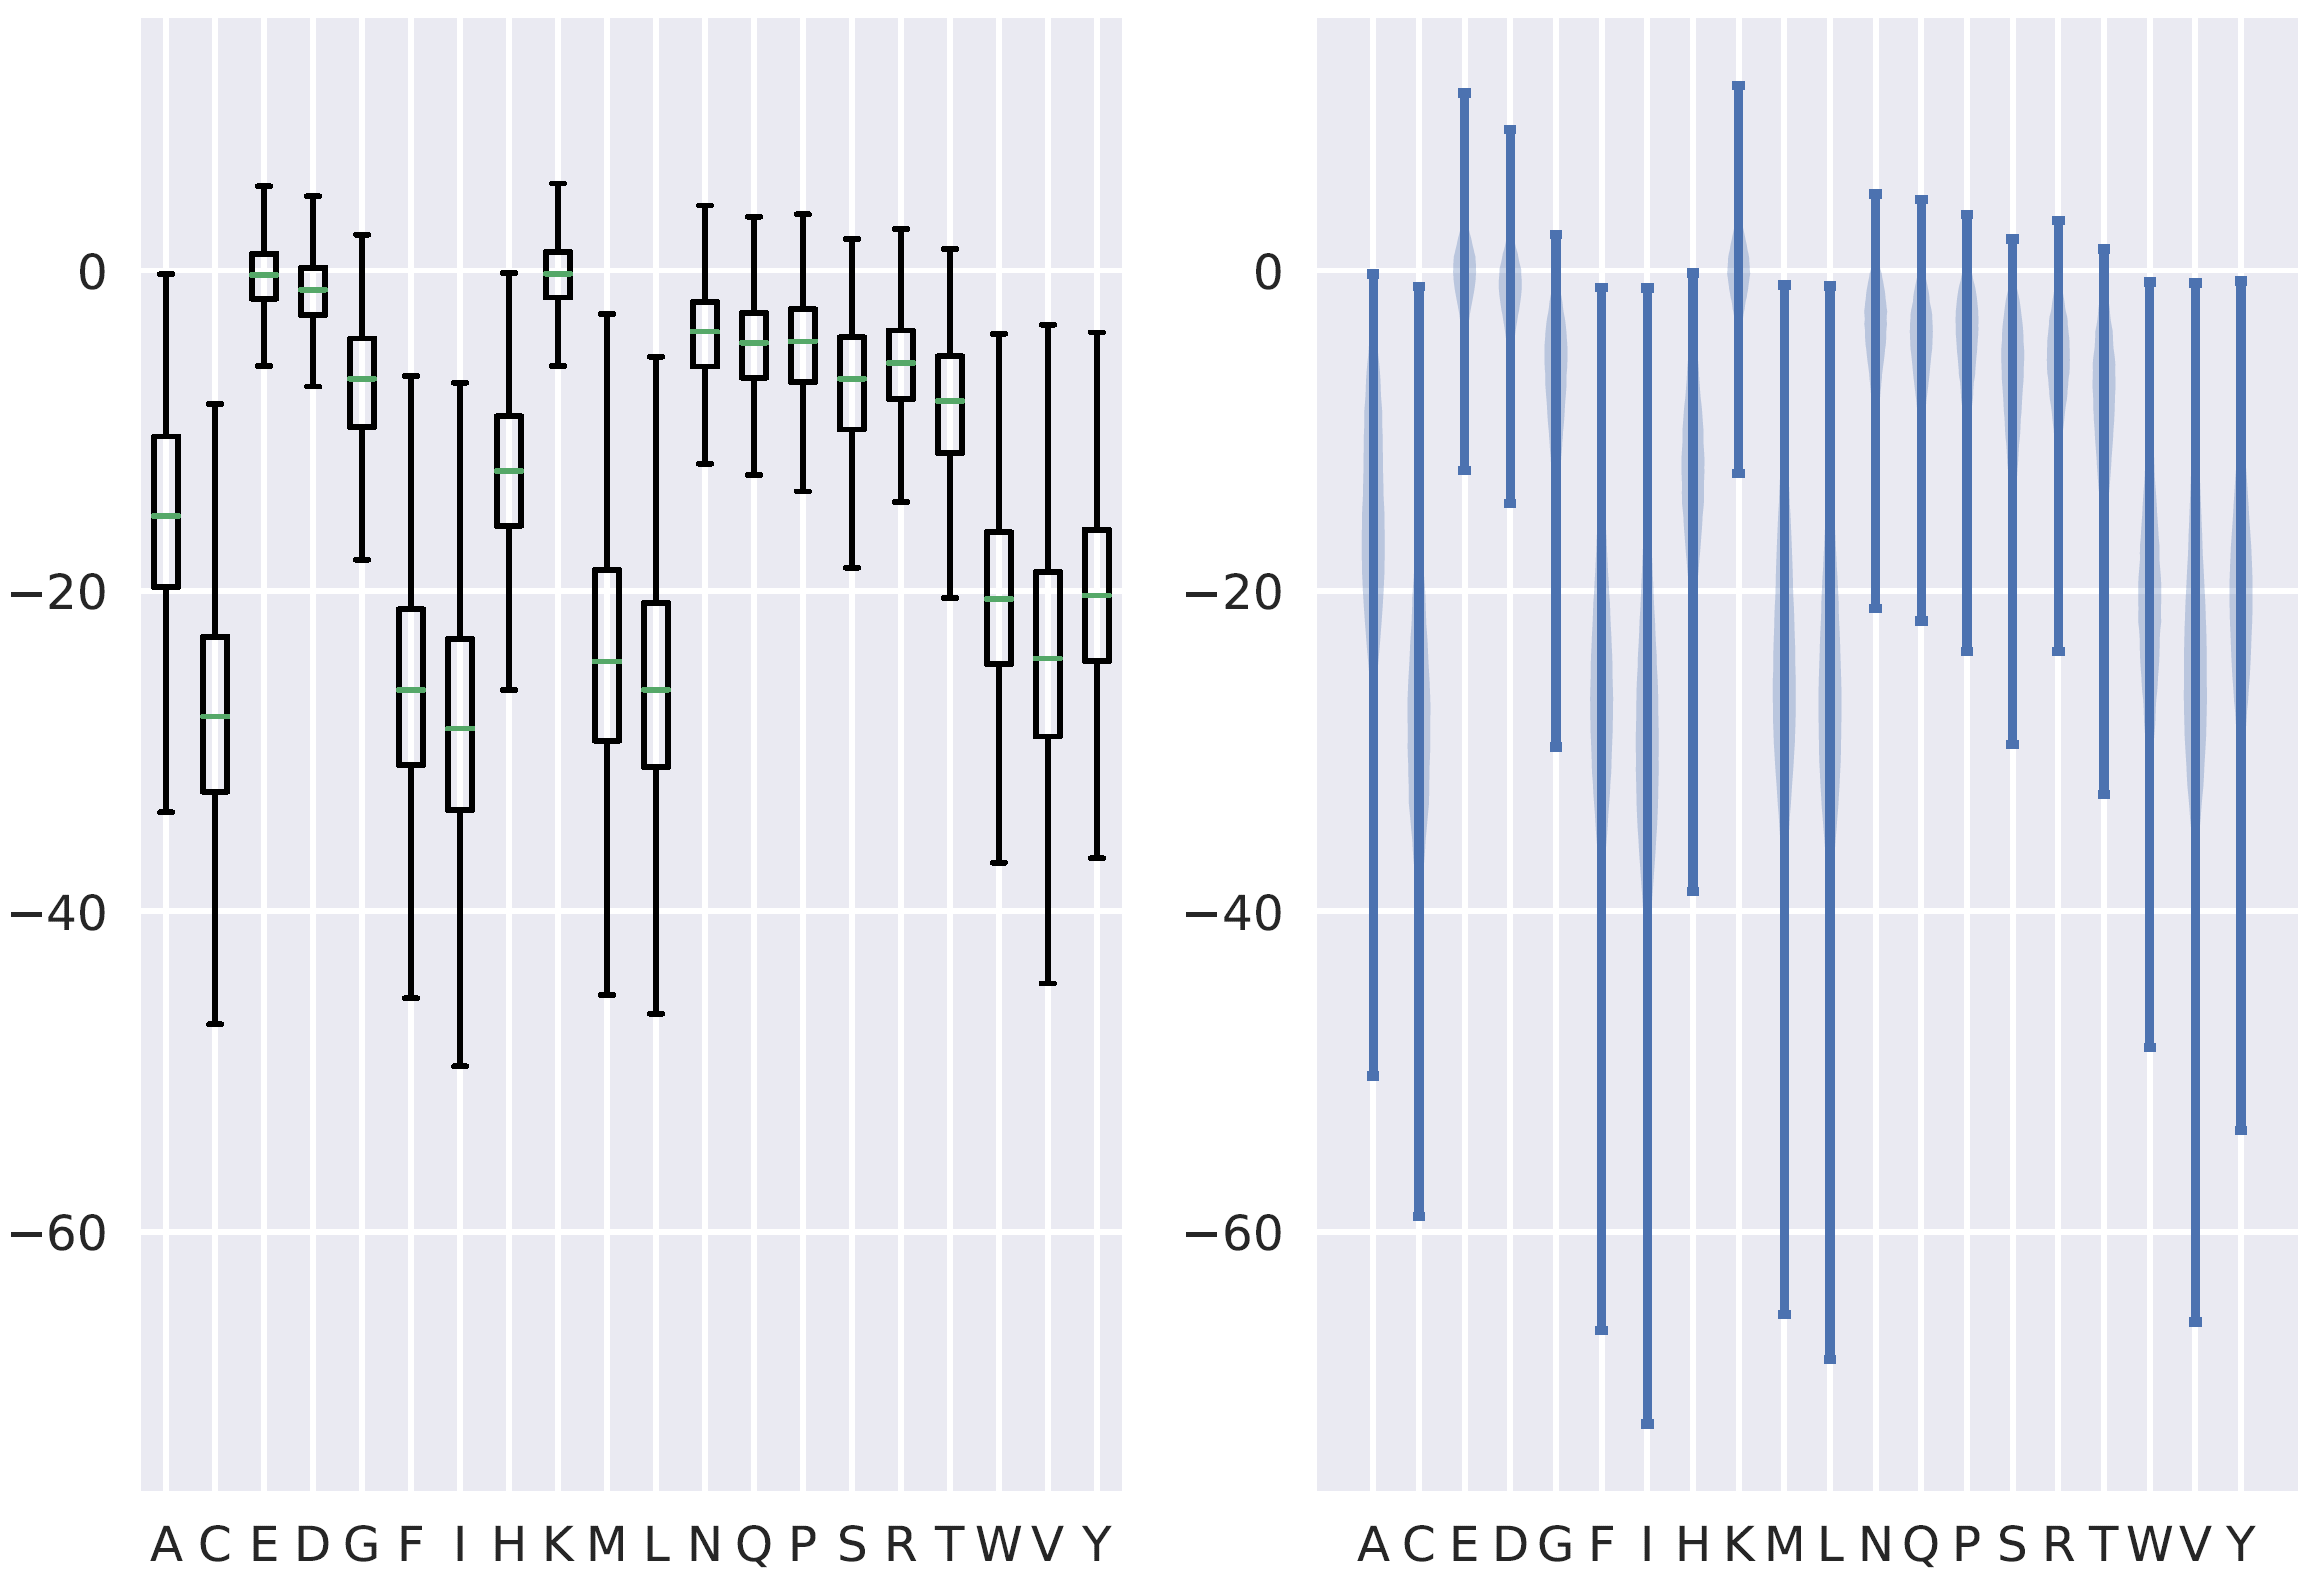
\includegraphics[width=.99\textwidth]{images/BoxPlot_energy_rages.png}
    \caption{Energien pro Aminosäure im Boxplot links und Violin Plot rechts dargestellt. Auf der Abszisse stellen die Buchstaben Abkürzungen der einzelnen Aminosäuren dar, siehe Tabelle \ref{tab:amino_table}. Auf der Ordinate sind die Energiewerte aufgetragen. Bei dem Boxplot wurden die Ausreißer mittels Grubbs-Test entfernt.}
    \label{fig:energy_ranges}
\end{figure}

Zum Beispiel reicht das Spektrum der \ac{APs} von Glutaminsäure und Asparaginsäure von etwa -6 bis +6, während sich das Spektrum von Phenylalanin und Isoleuchin von -50 bis -6 bewegt. 

Zusätzlich zum Boxplot wurde noch ein Violinen Plot für jede Aminosäure erstellt. Dieser zeigt nochmals die Verteilung der Energiewerte innerhalb einer Aminosäure. Es ist so deutlich zu sehen, dass alle Werte um einen Mittelwert verteilt sind, sowie das die Anzahl der Werte stark abflacht sobald man sich den äußeren Bereich des jeweiligen Spektrums nähert.

Der Violinen Plot beinhaltet zudem noch alle Ausreißer, aufgrund dessen sich das Spektrum im allgemeinen länger darstellt, als es im Boxplot der Fall ist. Die Ausreißer wurden im Boxplot mit Hilfe des Grubbs Test\cite{Jain.2010} herausgefiltert. 


\subsection{Spektrum der Aminosäuren im Detail}
In diesem Abschnitt wird das Spektrum der zwei Aminosäuren, Glutaminsäure und Glycin im Detail vorgestellt. Diese beiden Aminosäuren wurden exemplarisch Ausgewählt, da sich alle Aminosäuren Spektren ähnlich verhalten. So ist in \ac{Abb} \ref{fig:ep_as_distr} deutlich zu sehen das alle Enerigewerte der Glutaminsäure um einen Mittelwert (-0.1) verteilt sind. Dies verhält sich sehr ähnlich für Glycin, hier sind ebenfalls alle Werte um den Mittelwert (-5.1) verteilt. Jedoch fällt auf, dass die Kurve nicht ganz symmetrisch ist, wie in der Verteilung von Energiewerten der Glutaminsäure, sondern nach links flacher abfällt. Die Verteilungen wurden mit dem Skript \texttt{check\_aa\_energy\_range.py} erstellt, die restlichen \ac{Abb} sind im Anhang dieser Arbeit zu finden. 

Ein Test auf Normalverteilung aus dem Python Packet \emph{scipy}\footnote{\url{https://docs.scipy.org/doc/scipy/reference/generated/scipy.stats.mstats.normaltest.html}} hat ergeben, dass die Energie Werte nicht normal Verteilt sind, da die Kurve eine zu geringe Varianz aufweist. 

\begin{figure} 
    \subfigure[\ac{AP} Verteilung von Glutaminsäure]{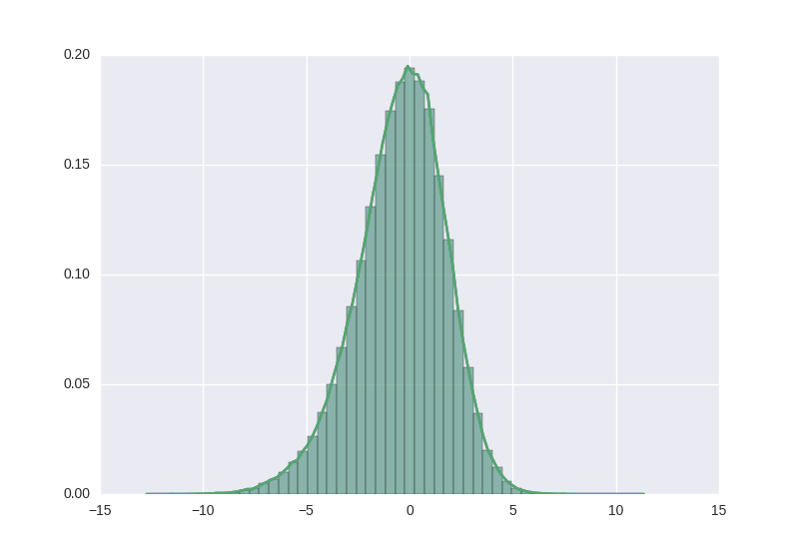
\includegraphics[width=0.49\textwidth]{images/Glutaminsaure_distr.png}}
    \subfigure[\ac{AP} Verteilung von Glycin]{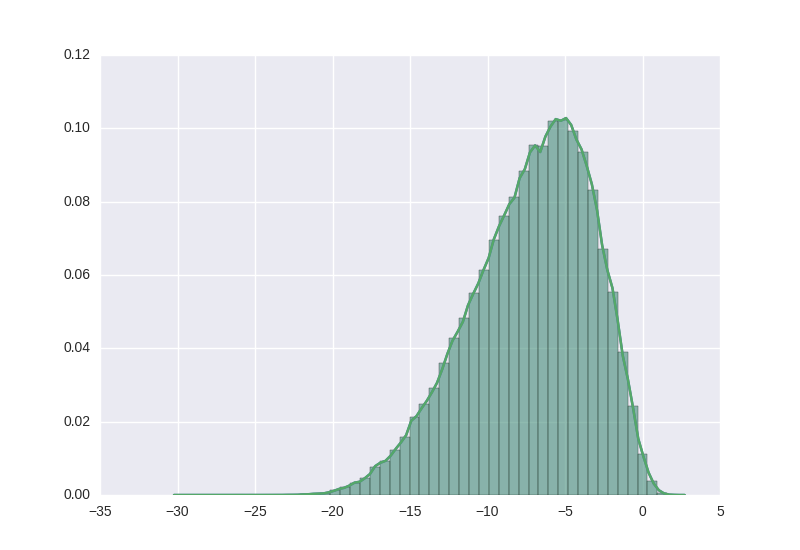
\includegraphics[width=0.49\textwidth]{images/histogramm_G.png}}
    \caption{Distribution der Energiewerte von Glutaminsäure links und Glycin rechts. Auf der Abszisse sind die Energiewerte aufgetragen und auf der Ordinate ihr relatives Vorkommen als Dezimalzahl.} 
    \label{fig:ep_as_distr}
\end{figure} 


\newpage
\section{SNP Analysen mittels EPs}
\label{sec:snp_analyse}

Um eine eine Aussage über die eventuelle Pathogenität von \ac{SNP}s zu treffen, war es erforderlich geeignete \ac{SNP}s zu finden, die betreffenden Gene zu identifizieren, eine \ac{PDB} Datei mit den Strukturinformationen des betreffenden Proteins zu haben und anschließend das Energieprofil für die generierten \ac{PDB} Dateien zu berechnen. Damit die \ac{EP}s anschließend vergleichen und ausgewertet werden können.


\subsection{Identifizierung der SNPs}

Um geeignete \ac{SNP}s für eine aussagekräftige Analyse zu finden, wurde auf die Datenbank ClinVar\footnote{\url{https://www.ncbi.nlm.nih.gov/clinvar/}} zurück gegriffen. Diese enthält Daten über genetische Variationen und die Auswirkungen auf die menschliche Gesundheit. Zum Zeitpunkt dieser Arbeit (Oktober 2017) enthielt sie 82.147 als \emph{pathogenic} markierte und 105.337 als \emph{benign} markierte genetische Variationen. Jedoch konnte nicht ohne weiteres aus diesem Datensatz geschöpft werden, denn viele Variationen enthalten widersprüchliche Annotationen. Um die Qualität der Annotation zu bewerten gibt es den sogenannten \emph{Review Status} dieser gibt an, wie gut die Annotation ist. So gibt es z.B. einen Stern, wenn die genetische Variation bisher nur von einem Autoren eingetragen wurde. Gibt es mehrere Autoren und widersprechen sich die Annotationen nicht, so bekommt die Annotation zwei Sterne. Die fast beste Qualität, mit drei Sternen, hat das \emph{expert panel}, Autoren in dieser Kategorie müssen spezielle Anforderungen erfüllen\footnote{\url{https://www.ncbi.nlm.nih.gov/clinvar/docs/review_guidelines/}}. Die beste Annotation mit vier Sternen hat \emph{practice guideline}, jedoch fallen fast keine \ac{SNP}s (23) in diese Kategorie, aus diesem Grund wurden erst nur Variationen betrachtet, welche aus dem \emph{expert panel} kommen. 
%
\begin{table}[]
    \centering
    \caption{Tabelle aller Gene des \emph{expert panels} mit mindestens 10 Pathogenen \ac{SNP}s. Die verwendeten Gene sind grün markiert.}
    \label{tab:expert_snps}
    \resizebox{\linewidth}{!}{%
    \begin{tabular}{llllllll}
    \hline
    \multicolumn{1}{|l|}{Name} & \multicolumn{1}{l|}{Template} & \multicolumn{1}{l|}{Länge} & \multicolumn{1}{l|}{Coverage} & \multicolumn{1}{l|}{Identity} & \multicolumn{1}{l|}{QMEAN} & \multicolumn{1}{l|}{SNPs} & \multicolumn{1}{l|}{Assozierung} \\ \hline
    \rowcolor[HTML]{9AFF99} 
    MSH2 & 3thw.1.A & 934 & 98,40\% & 100\% & -2,05 & 33 & globulär \\ \hline
    \multicolumn{1}{|l}{BRCA1} & 1jm7.1.A & 1863 & 5,50\% & 100\% & -0,13 & 24 & \multicolumn{1}{l|}{globulär} \\
    \multicolumn{1}{|l}{} & 4y18.1.A &  & 11,40\% &  & -2,18 &  & \multicolumn{1}{l|}{} \\ \hline
    BRCA2 & 1miu.1.B & 3418 & 21\% & 75,48\% & -5,05 & 10 & globulär \\
    \rowcolor[HTML]{9AFF99} 
    CFTR & 5uak.1.A & 1480 & 96,70\% & 100\% & -4,51 & 44 & membran \\
    MYH7 & 5tby.1.A & 1935 & 49,50\% & 100\% & -4,8 & 32 & globulär \\ \hline
    \multicolumn{1}{|l}{MLH1} & 4p7a.1.A & 756 & 44\% & 100\% & -0,73 & 65 & \multicolumn{1}{l|}{globulär} \\
    \multicolumn{1}{|l}{} & 3rbn.1.A &  & 34,90\% & 100\% & -1,29 &  & \multicolumn{1}{l|}{} \\ \hline
    \end{tabular}}
\end{table}

Das \emph{expert panel} enthält 5.437 pathogene und 2.878 gutartige Variationen, von diesen waren 1.717 und 2.697 \ac{SNP}s für diese Arbeit von Interesse, die anderen genetischen Variationen aus Deletionen, Duplikationen und Insertionen bestehen. Ausgehend von diesen \ac{SNP}s wurden alle Gene ausgewählt welche mindestens 10 Pathogene SNPs in der ClinVar besitzen. So wurden 6 Gene ausgewählt und die Aminosäure Sequenz aus der NCBI Protein Datenbank\footnote{\url{https://www.ncbi.nlm.nih.gov/protein/}} heruntergeladen und für jeden \ac{SNP}s eine Sequenz angelegt. 

\begin{table}[]
    \centering
    \caption{Tabelle aller Gene der ClinVar Datenbank, mit mindestens 6 Pathogenen SNPs und multiplen Autoren, ohne Widerspruch. Die Verwendeten Gene mit guter Sequenzidentität und Coverage sind grün markiert. Die Gene welche noch ausreichende Sequenzidentität und Coverage aufwiesen sind hell grün markiert.}
    \label{tab:multiple_subs_snps}
    \resizebox{\linewidth}{!}{%
    \begin{tabular}{llllllll}
    \hline
    \multicolumn{1}{|l|}{Name} & \multicolumn{1}{l|}{Template} & \multicolumn{1}{l|}{Länge} & \multicolumn{1}{l|}{Coverage} & \multicolumn{1}{l|}{Identity} & \multicolumn{1}{l|}{QMEAN} & \multicolumn{1}{l|}{SNPs} & \multicolumn{1}{l|}{Assozierung} \\ \hline
    MFN2 & 5gom.1.A & 757 & 51,30\% & 71.21\% & -1,32 & 13 & globulär \\
    \rowcolor[HTML]{CBFFCB} 
    SDHB & 1zoy.1.B & 280 & 85,70\% & 97.54\% & -0,88 & 10 & Membran \\
    MUTYH & 3n5n.2.A & 535 & 51,40\% & 100\% & -1,8 & 14 & globulär \\
    ALPL & 1zef.1.A & 524 & 90\% & 58,58\% & -2,04 & 8 & globulär \\
    \rowcolor[HTML]{9AFF99} 
    SLC2A1 & 4pyp.1.A & 492 & 90,70\% & 99,59\% & -4,75 & 8 & Membran \\
    \rowcolor[HTML]{9AFF99} 
    ACADM & 1ege.1.B & 421 & 91,70\% & 100\% & -1,23 & 11 & globulär \\
    LMNA & 1ufg.1.A & 572 & 22,70\% & 96,18\% & -4,66 & 21 & globulär \\
    ABCA4 & 5xjy.1.A & 2273 & 98,90\% & 51,97\% & -6,57 & 22 & Membran \\
    TNNT2 & 1j1d.2.B & 295 & 25,10\% & 99,03\% & 0,87 & 10 & globulär \\
    COL9A2 & 5ctd.1.B & 689 & 6,30\% & 86,67\% & 0,41 & 6 & globulär \\
    STIL & 4yyp.1.B & 1288 & 100\% & 2\% & -0,03 & 6 & globulär \\
    AGL & 5d06.2.A & 1532 & 43,09\% & 97,30\% & -4,43 & 8 & globulär \\
    \rowcolor[HTML]{CBFFCB} 
    KCNQ1 & 5vms.1.A & 676 & 68,50\% & 83,30\% & -5,87 & 10 & Membran \\
    \rowcolor[HTML]{CBFFCB} 
    KCNH2 & 5va2.1.A & 1159 & 74,20\% & 96,56\% & -5,38 & 6 & Membran \\
    PMS2 & 1h7s.1.A & 862 & 39\% & 100\% & 0,25 & 6 & globulär
    \end{tabular}}
\end{table}

Da der Datensatz erst 6 Gene umfasst, wurden die Kriterien der \ac{SNP} Auswahl erweitert. So wurden in einem zweiten Durchlauf auch jende \ac{SNP}s hinzugezogen, welche nicht im \emph{expert Panel} waren, sondern lediglich von mehreren Autoren eingetragen wurden. Somit standen 3.826 pathogene und gutartige 19.070 \ac{SNP}s zu Verfügung. Des weiteren wurde die Mindestanzahl an pathogener SNPs auf 6 pro Gen verringert. So konnte der Datensatz um 15 Gene erweitert werden, siehe Tabelle \ref{tab:multiple_subs_snps}.


\subsection{Homologie Berechnungen}

Sobald alle Proteine mit den \ac{SNP}s vorlagen musste eine Homologie Modellierung durchgeführt werden. Denn zum Einen besitzen nicht alle Proteine eine aufgeklärte Struktur und zum Anderen sind nur sehr wenige mutierte Proteine strukturell aufgeklärt. So war es notwendig jeweils für das Proteine und die Mutation mit dem \ac{SNP} eine Homologie Berechnung durchzuführen. Hierzu wurde wie in Kapitel \ref{sec:siwssmodel} gezeigt mit Swissmodel eine Berechnung durchgeführt.

Die Ergebnisse sind in \ref{tab:expert_snps} dargestellt, wie zu sehen ist, ist die größte Coverage bei \texttt{MSH2} mit 98,4\% gefolgt von \texttt{CFTR} mit 96,7\%. Die Sequenz Identität beträgt bei beiden 100\%. Bei fast allen Sequenzen wurden mehrere Templates gefunden, doch meist weisen die Meisten eine sehr niedrige Coverage auf, sodass sie hier nicht dargestellt sind. Bei \texttt{MLH1} wurden zwei Templates gefunden, welche 44\% und 34,9\% der Sequenz abdecken. Bei \texttt{BRCA1} wurden ebenfalls mehrere Templates gefunden, so dass hier eine Coverage von 11,4\% und 5,5\% vorliegt. \texttt{BRCA2} hat eine Coverage von 21\% bei 75,48\% Sequenzidentität.

In einem zweiten Durchgang wurden auch alle Proteine mit ihren SNPs aus \ref{tab:multiple_subs_snps} mittels Swissmodel strukturell modelliert. Hierbei zeigte \texttt{ABCA4} die höchste Coverage, doch nur eine Sequenzidentität von 51,97\%. Betrachtet man Coverage und Sequenzidentität, so weisen \texttt{SLC2A1} und \texttt{ACADM} die höchste Coverage mit 90,7\% und 91,7\% auf. 

\textbf{die Tabellen noch mehr erklären?} JAA 



\subsection{Berechnung \& SNPs in Energieprofilen}

Nachdem nun die \ac{PDB} Dateien vorliegen, wurde für jede dieser Dateien ein Energieprofil berechnet wie es auch in Kapitel \ref{sec:calc_ep} beschrieben ist. Diese \ac{EP}s wurden nun anschließend mit dem Skript \texttt{plot\_eps\_and\_snps.py} analysiert und geplottet. 
%
\begin{figure}
    \centering
    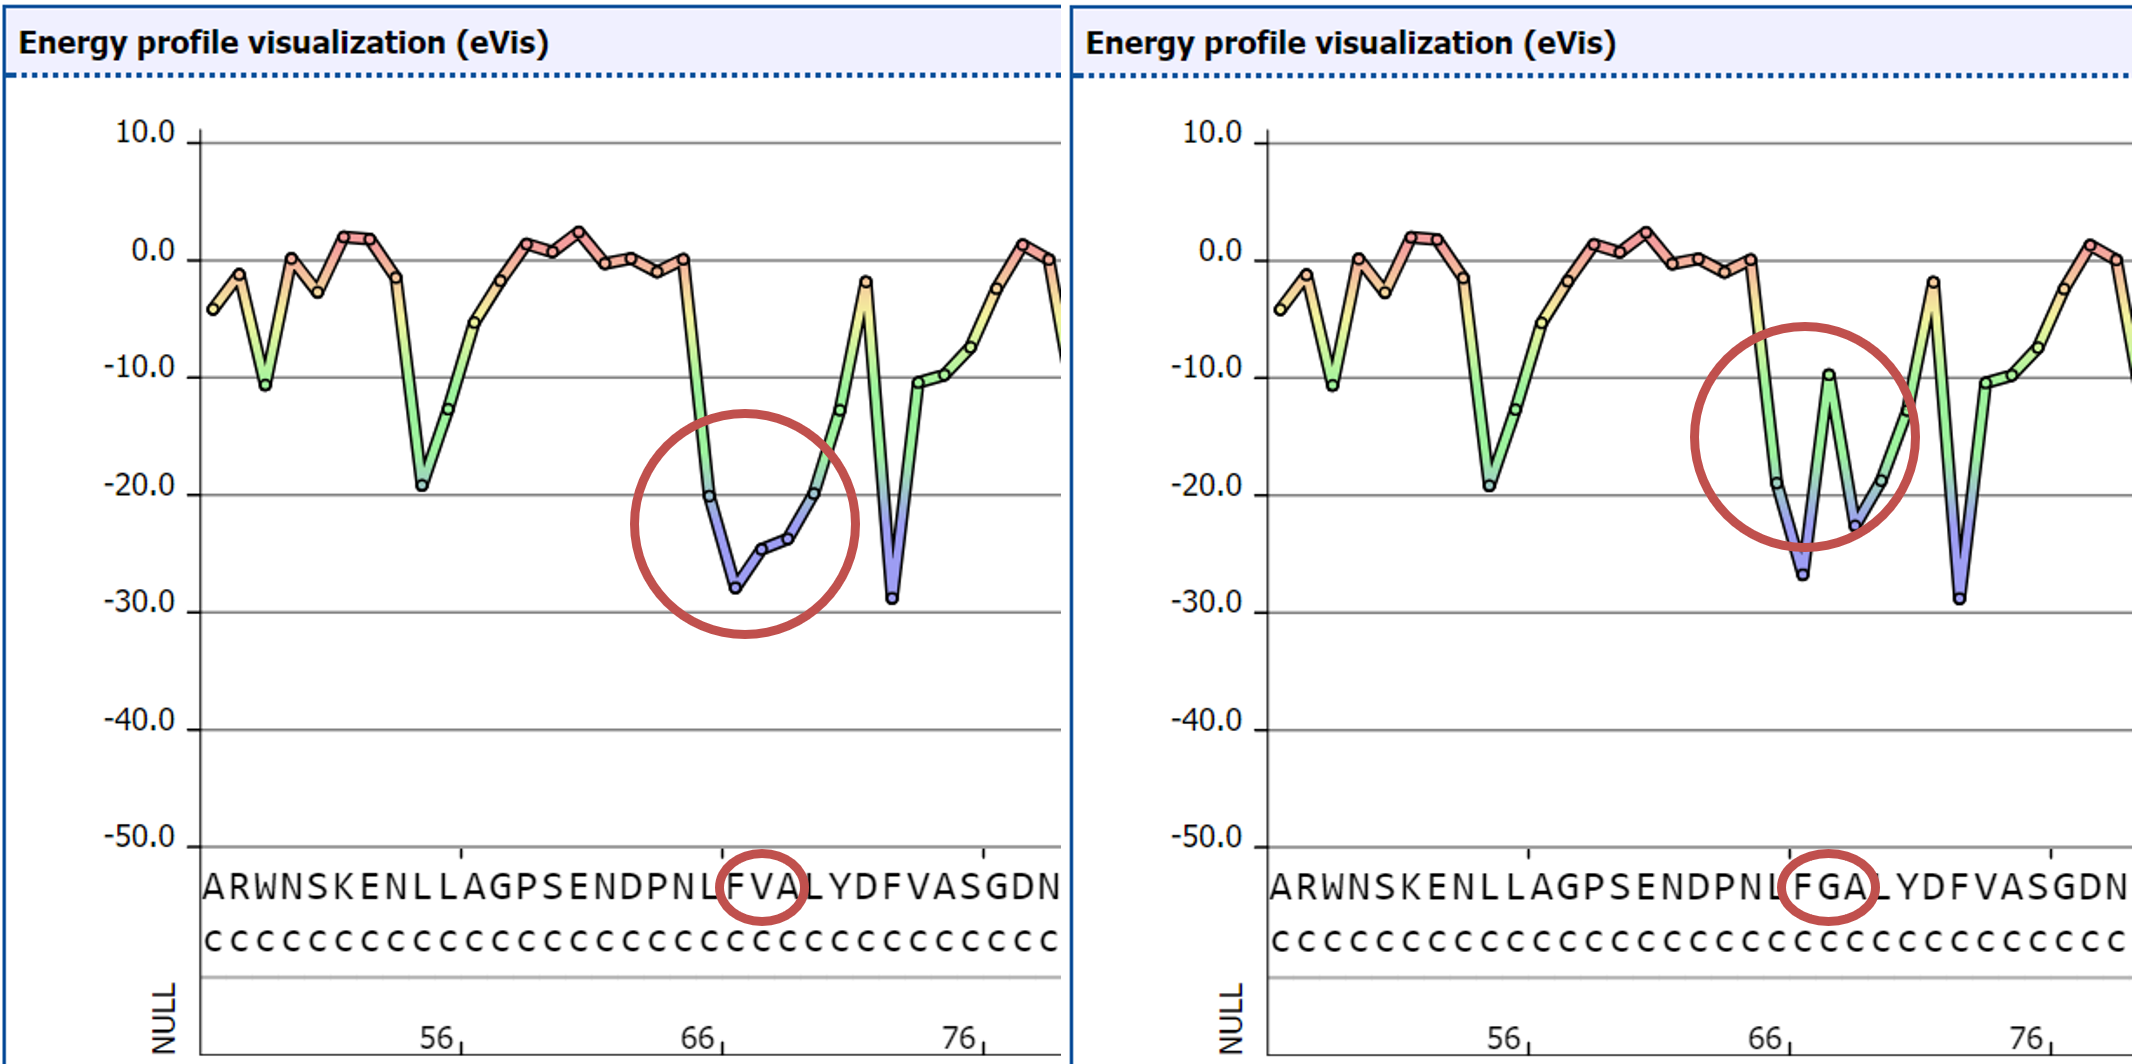
\includegraphics[width=.99\textwidth]{images/ep_vs_snp.png}
    \caption{\ac{eVis} Darstellung vom ePros Webserver (Kapitel \ref{sec:epros}) eines Ausschnittes eines \ac{EP}s. Die original Sequenz befindet sich links und Sequenz mit dem \ac{SNP}(rote Markierung) ist rechts. Auf der Abszisse sind die Aminosäuren im Einbuchstabencode aufgetragen, siehe Tabelle \ref{tab:amino_table}. Darunter ist die Sekundärstruktur als Buchstabencode und visualisiert aufgetragen. Unten ist die Aminosäureposition in 10er Schritten aufgetragen. Auf der Ordinate befinden sich die Energiewerte.}
    \label{fig:ep_vs_snp}
\end{figure}

Hierbei ist aufgefallen, dass sich die Energieprofile signifikant an den \ac{SNP} Positionen unterscheiden. Zum Verständnis ist ein \ac{EP} in \ac{Abb} \ref{fig:ep_vs_snp} dargestellt. Hier sieht man eine 2D Visualisierung eines \ac{EP}s, auf der Abszisse sind die Aminosäuren im Einbuchstabencode aufgetragen, wahrend auf der Ordinate die Energiewerte eingetragen sind. Die beiden Darstellungen unterscheiden sich nur durch die Substitution von Valin durch Glycin, so ist hier deutlich die Energiewert Differenz zwischen den beiden Darstellungen zu erkennen. So besitzt im Protein Valin an der Position 68 einen Energiewert von -25, der Glycin \ac{SNP} hingegen besitzt einen Energiewert von -10, so ergibt sich eine Delta von 15.

\begin{figure}
    \centering
    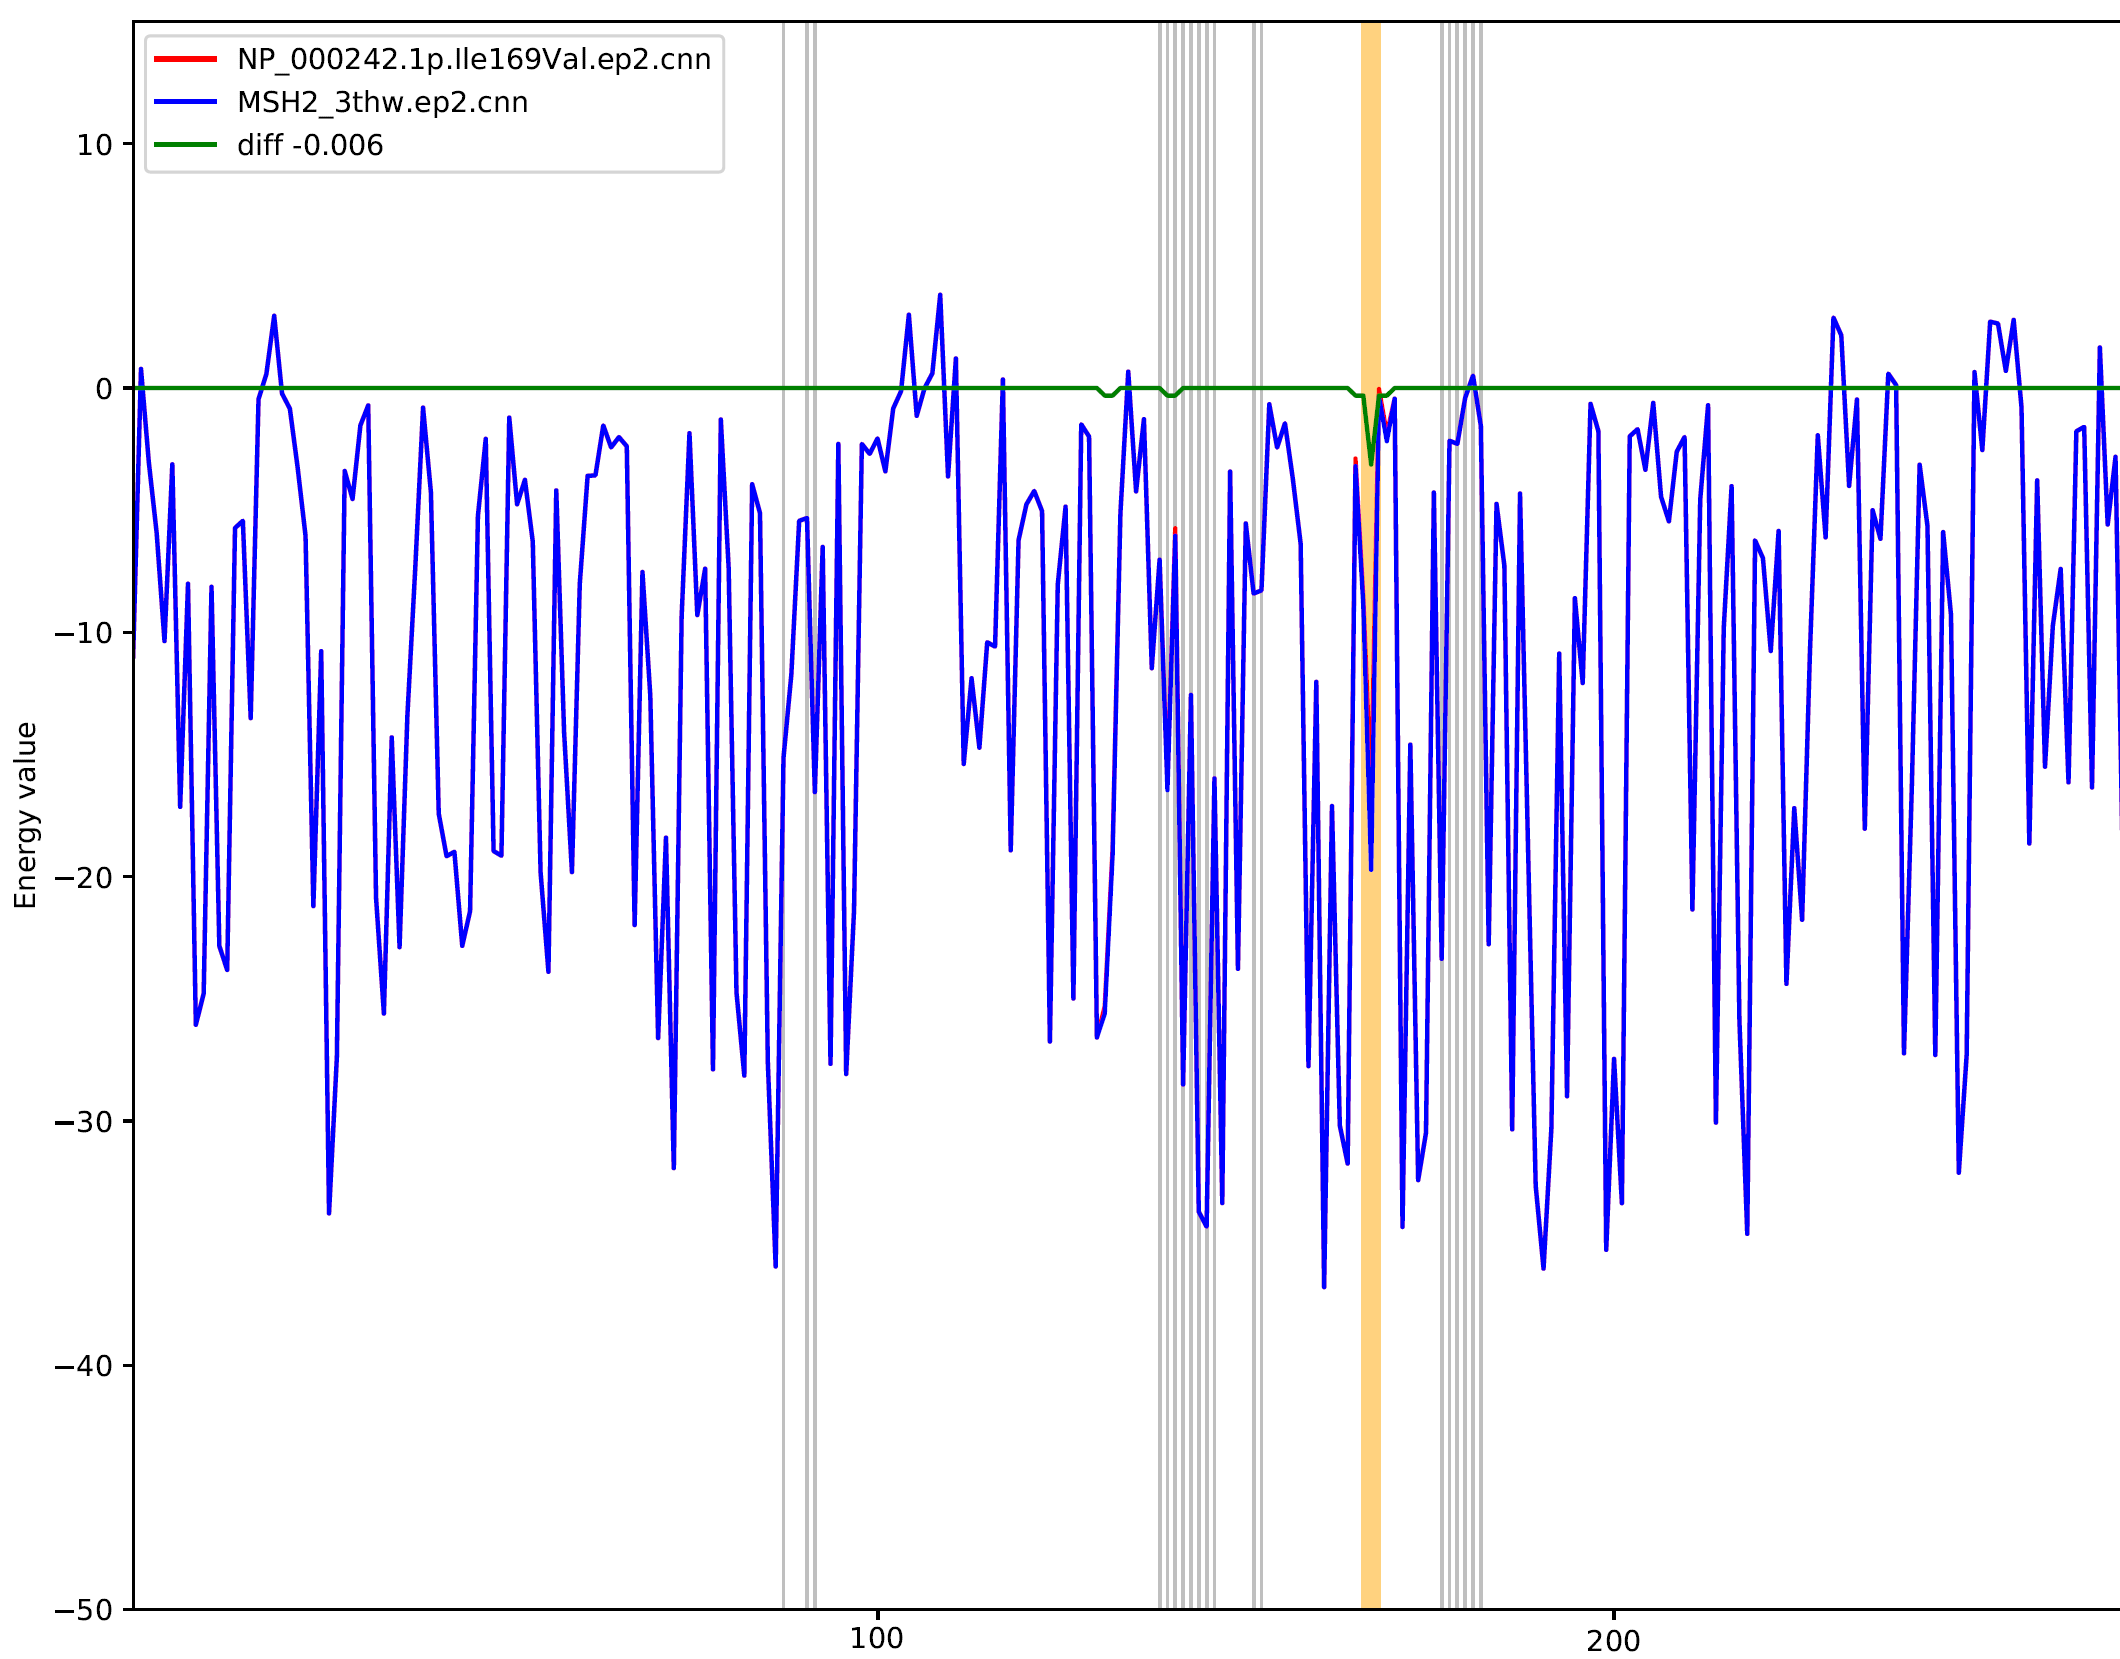
\includegraphics[width=.95\textwidth]{images/comp_plot_Ile169Val.png}
    %\caption{Ausschnitt aus dem Protein MSH2 mit gutartigem \ac{SNP} an Position 169.}
    %\label{fig:comp_plot_benign}
    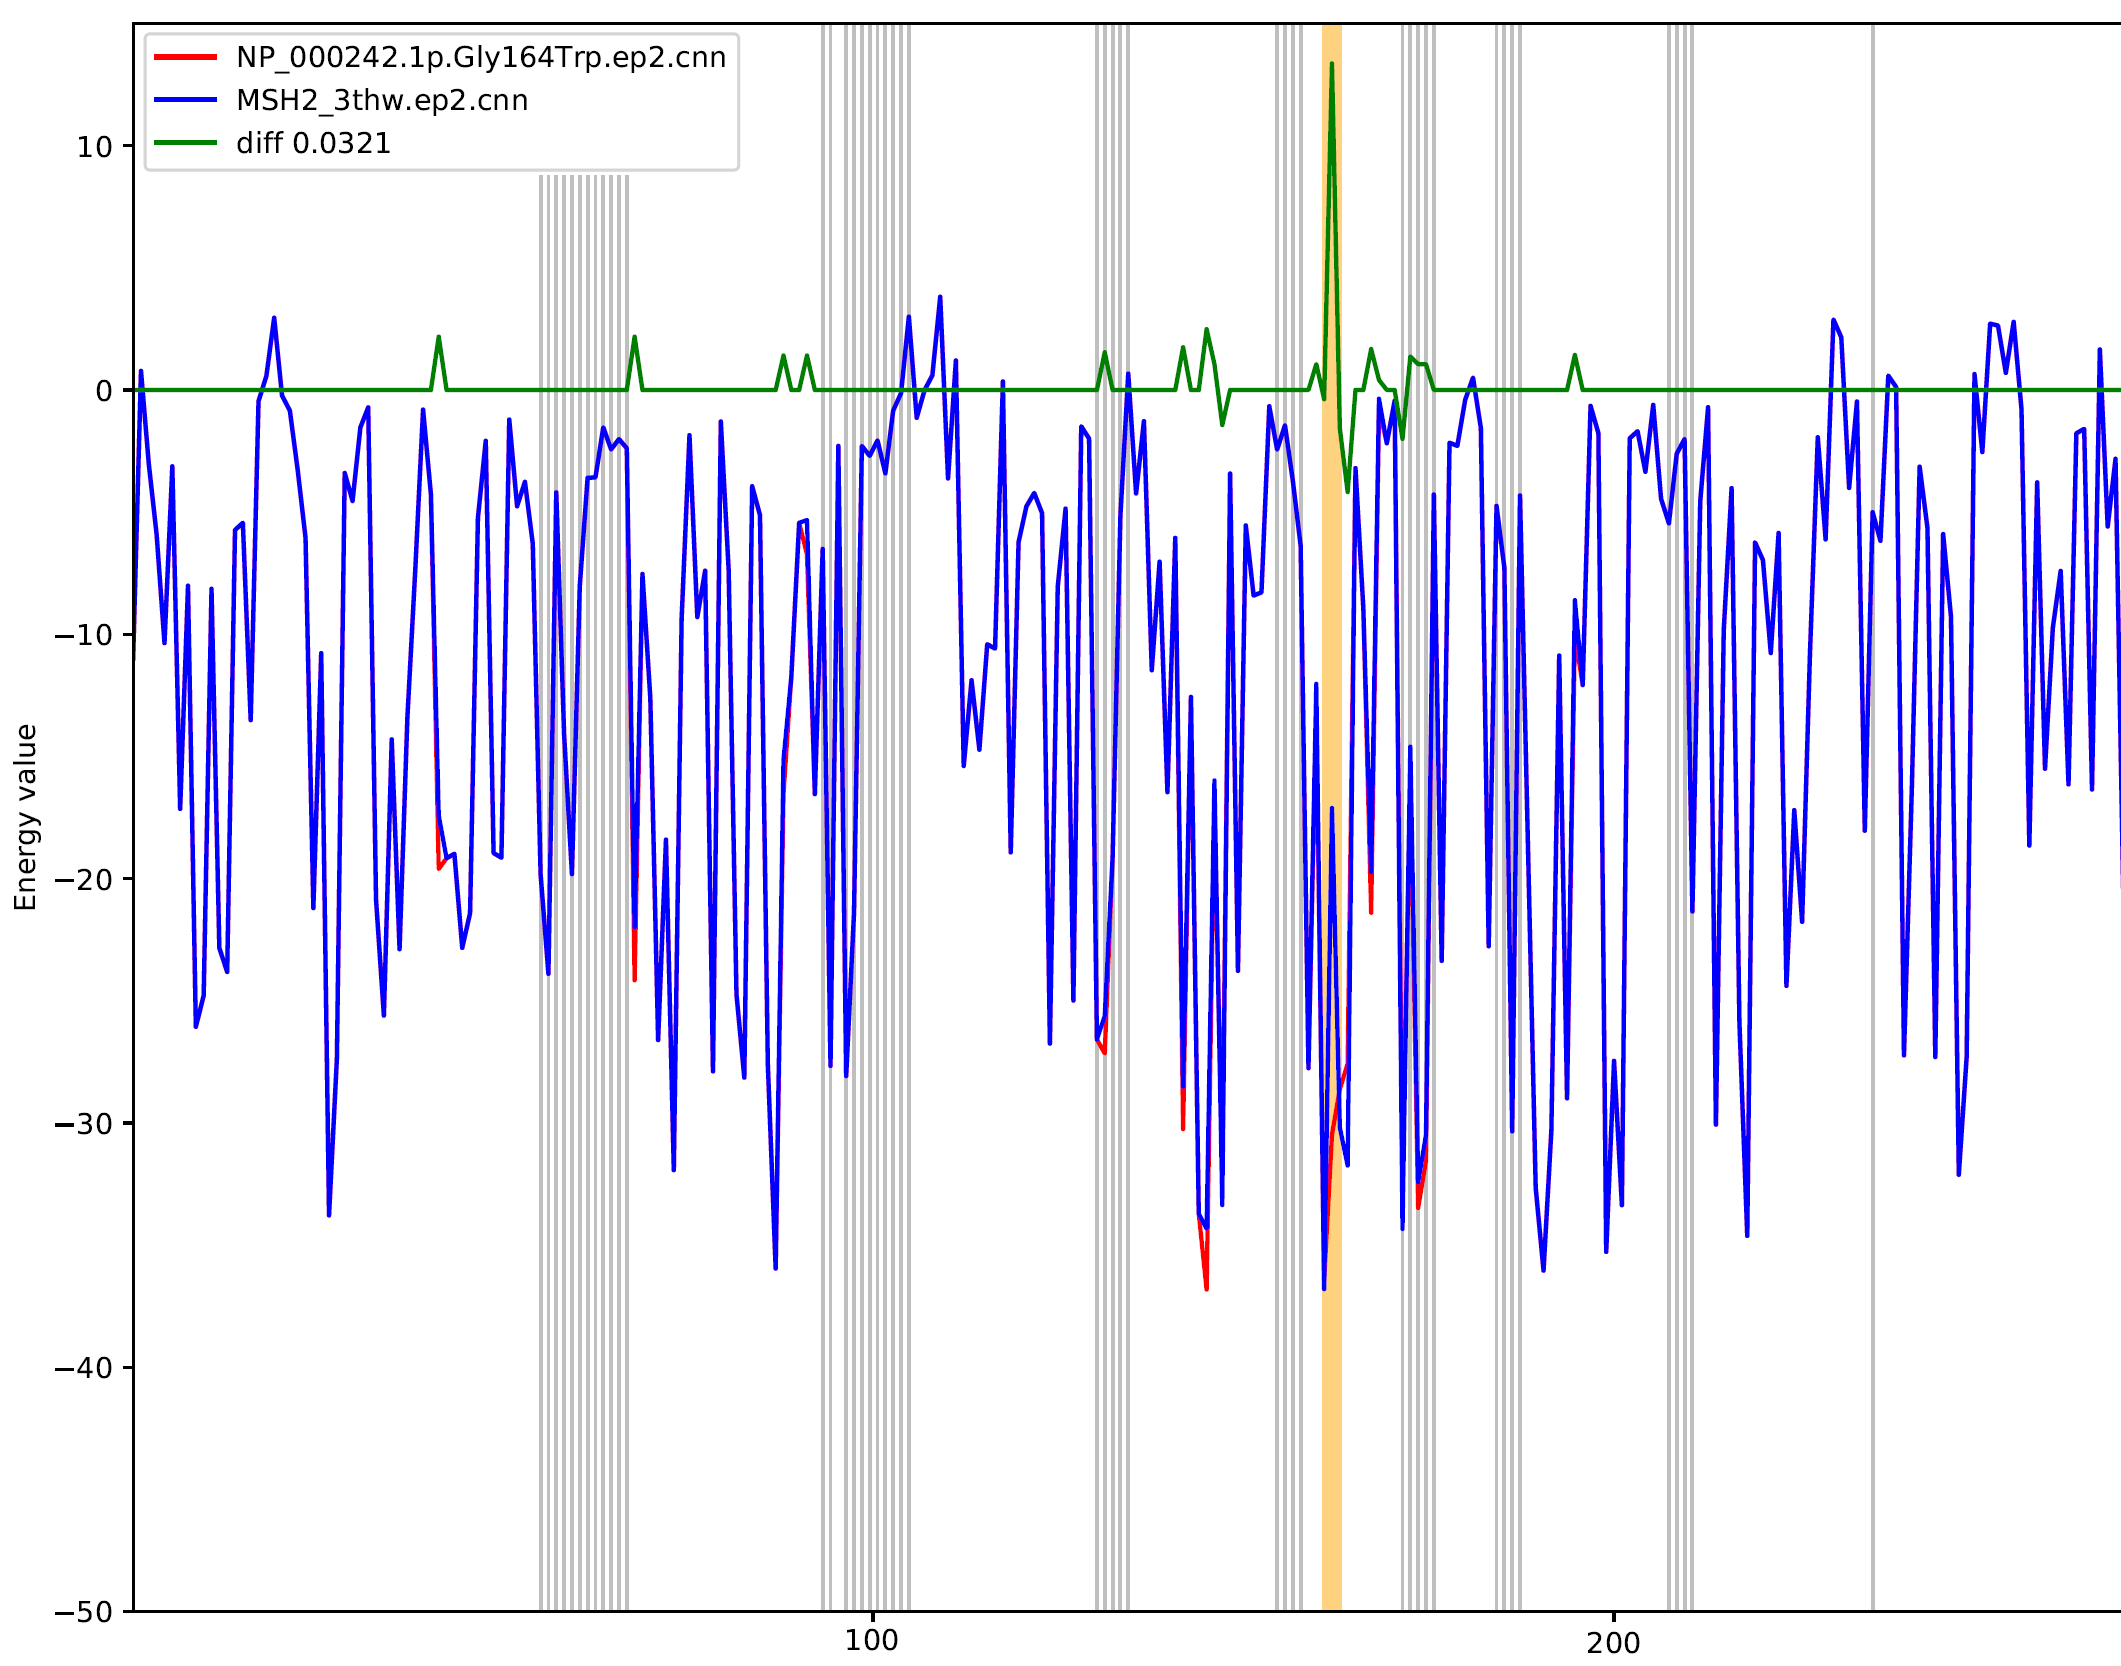
\includegraphics[width=.95\textwidth]{images/comp_plot_Gly164Trp.png}
    \caption{Ausschnitt aus dem Protein MSH2 mit gutartigem \ac{SNP} an Position 169 und mit pathogenen \ac{SNP} an Position 164.}
    \label{fig:comp_plot}
\end{figure}


Zudem wurden nicht nur Veränderungen unmittelbar am SNP festgestellt, sondern auch einige nicht ganz so starke Veränderungen an verschiedenen anderen Aminosäuren im Protein, auffällig hierbei ist, dass diese Veränderungen sehr oft an den vorher berechneten Kontakten der Aminosäure auftreten. 

In \ac{Abb} \ref{fig:comp_plot} ist ein beispielhafter Ausschnitt aus dem Protein \texttt{MSH2} dargestellt, die Abszisse gibt die Positionen der fortlaufenden Aminosäuren an, auf der Ordinate befinden sich die Energiewerte. Die Referenzsequenz ist blau dargestellt, die mutierte Sequenz ist rot dargestellt und die Differenz der beiden Sequenzen ist grün dargestellt. Die grauen Linien geben die Position der Kontakte an und die gelbe Linie zeigt die Position des \ac{SNP}s.

Im oberen Bild \ref{fig:comp_plot} ist an Position 169 eine Substitution von Isoleucin auf Valin zu sehen, der Energiewert an dieser Stelle wurde um etwa -2 verringert, an den Kontakten und generell in der gesamtem Sequenz, wurden nur sehr kleine Veränderungen festgestellt.

Im unteren Bild der \ac{Abb} ist eine Substitution an Position 164 von Glycin auf Tryptophan zu erkennen. Der Energiewert an dieser Position wurde um etwa 12 erhöht. Auffällig ist hierbei, dass sich auch die Kontakte verändert haben, generell lässt sich sagen, dass es im gesamten Protein zu energetischen Veränderungen kam.


\subsection{Auswertung der Energieprofile}

Da nicht alle SNPs innerhalb der aufgeklärten Struktur lagen, bestand der Datensatz am Ende aus 55 \ac{SNP}s aus den Genen \texttt{ACADM, CFTR, MSH2, PMS2} und \texttt{SDHB}. Nun wurde \ac{SNP}s nach Kriterien gesucht um diese SNPs zu trennen.


\textbf{in wie fern soll ich das hier noch ausführen? oder ist die Auswertung schon Diskussion}





\newpage
\section{PSI \& PHI Winkel Berechnung}

Der generierte Datensatz aus Kapitel \ref{sec:calc_ep}, ist Grundlage der folgenden Berechnung.

Bedingt durch die Tatsache das alle in dieser Arbeit \ref{sec:konst} gefilterten \ac{Pfam} auch eine aufgeklärte Struktur besitzen lies sich nun jede \ac{Pfam} in einen Ramachandran Plot darstellen, siehe \ac{Abb} \ref{fig:ramachandran_PF01287}.

% finde einen SNP der in der Pfam liegt und in der Clinvar ist

\begin{figure}
    \centering
    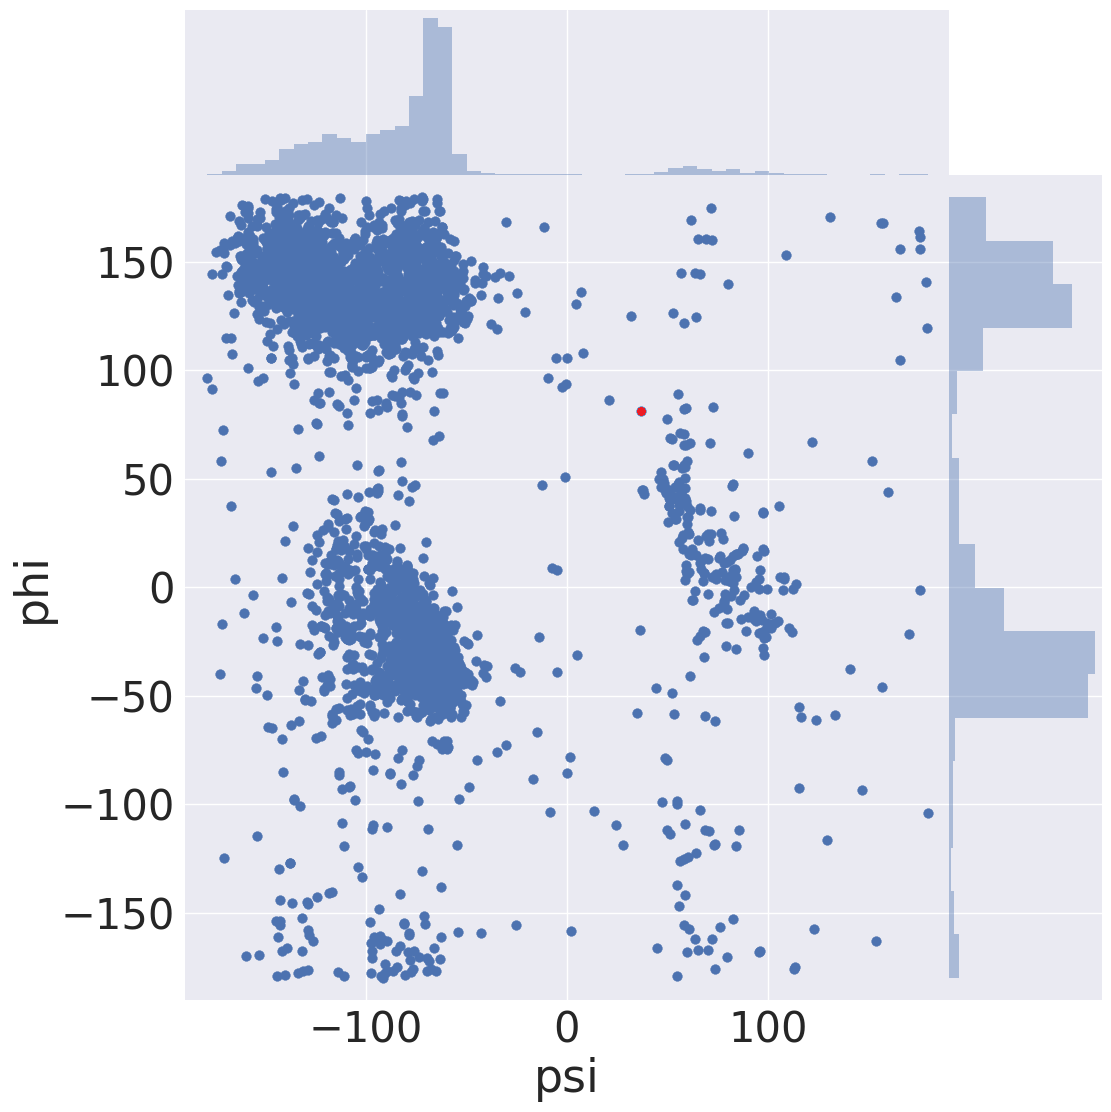
\includegraphics[width=.99\textwidth]{images/ramachandranplot_PF01287.png}
    \caption{Ramachandran Plot der Pfam PF01287}
    \label{fig:ramachandran_PF01287}
\end{figure}


Es treten nicht nur spezifische PSI und PHI Winkel auf, sondern fast im kompletten Spektrum des möglichen.

\begin{figure}
    \centering
    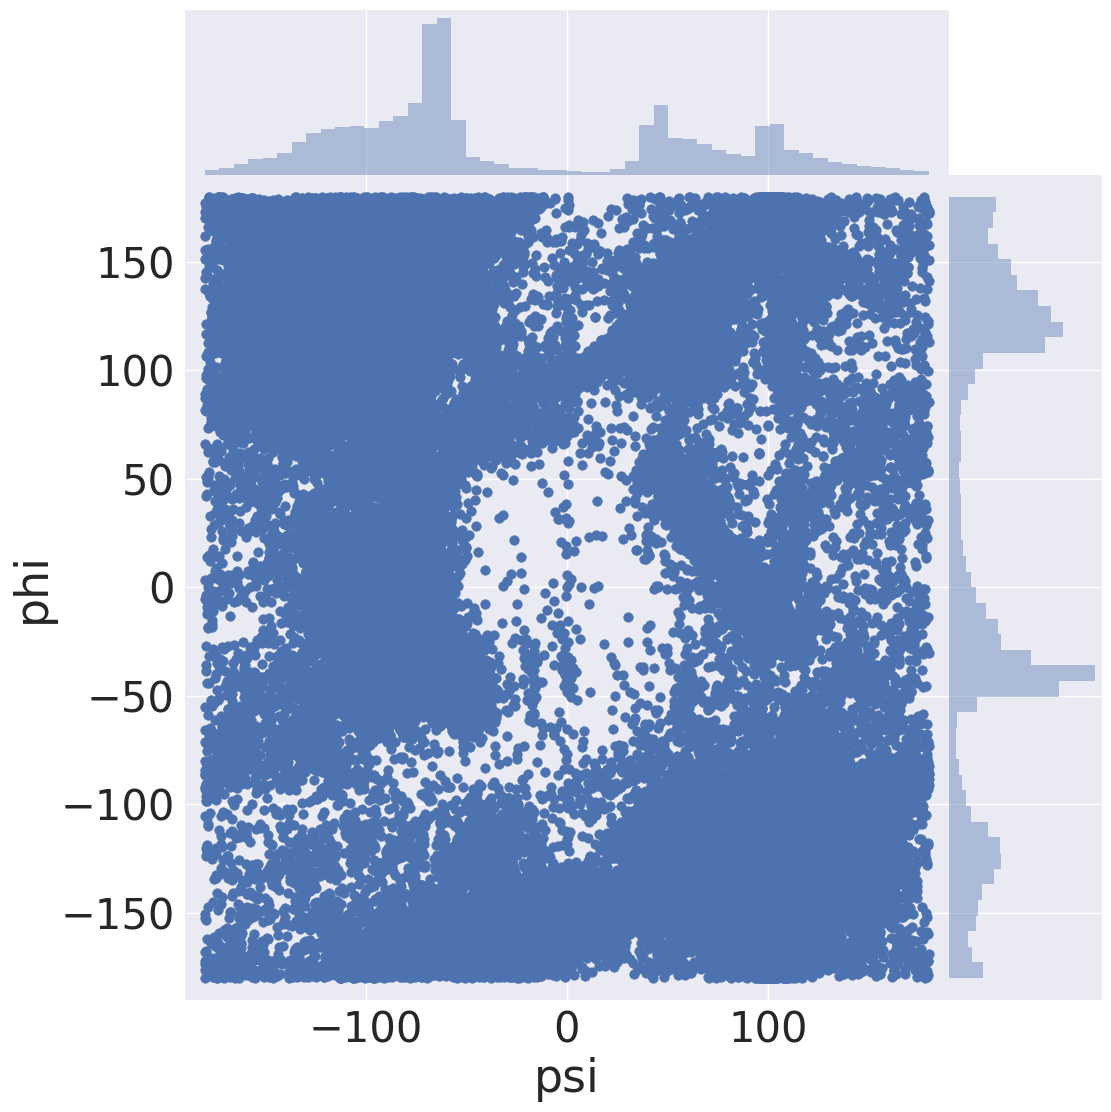
\includegraphics[width=.99\textwidth]{images/ramachandranplot_PF00883.png}
    \caption{Ramachandran Plot der Pfam PF00883}
    \label{fig:ramachandran_PF00883}
\end{figure}





